\documentclass[tikz,border=10pt]{standalone}
\usetikzlibrary{trees,positioning,arrows.meta,shadows.blur}

\begin{document}
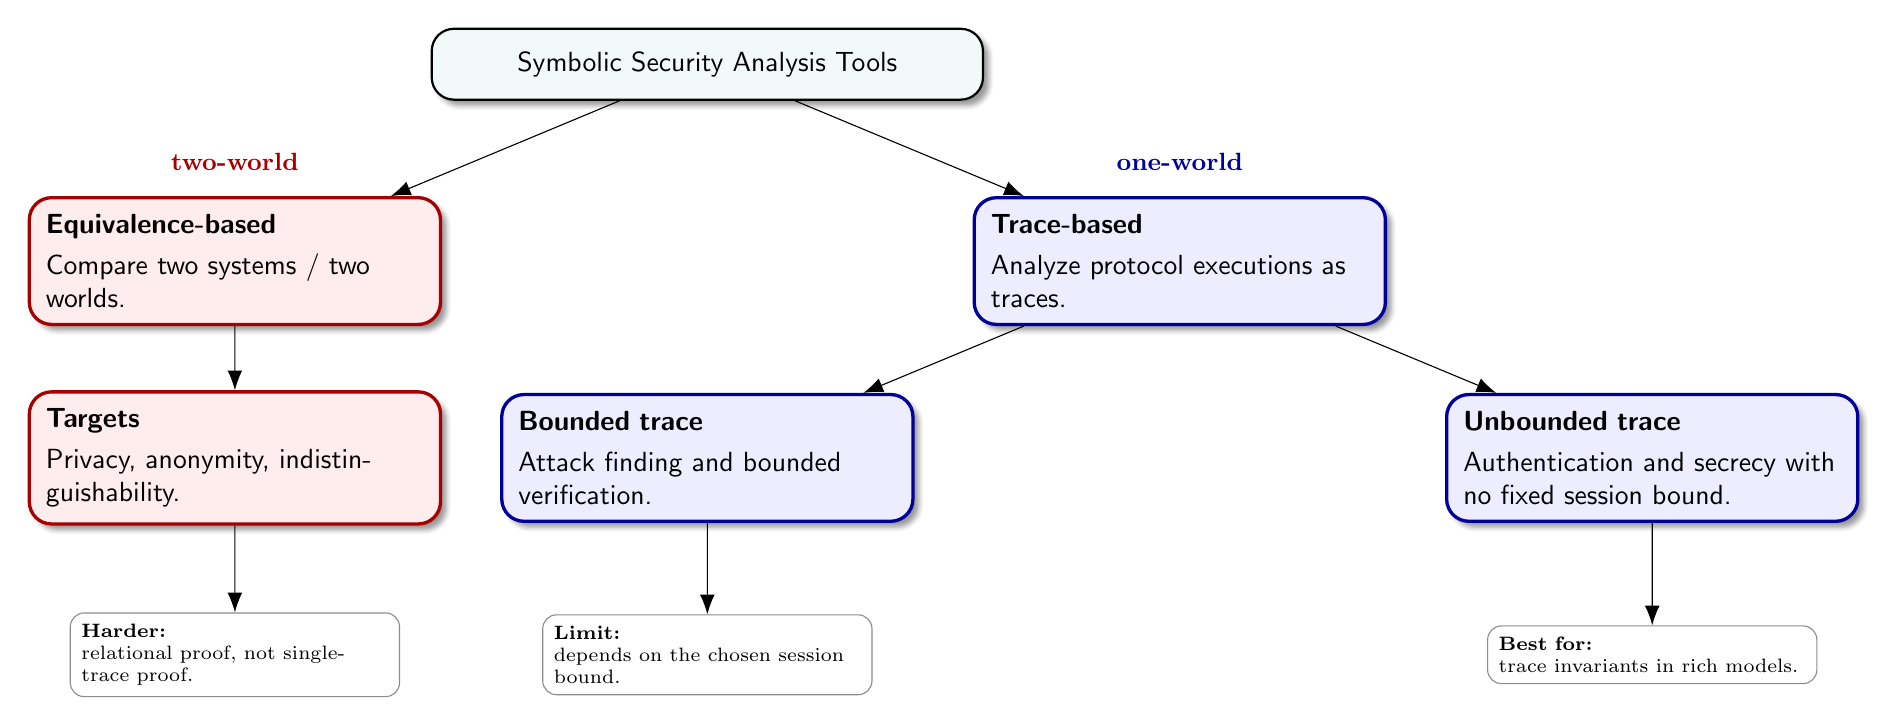
\begin{tikzpicture}[
	font=\sffamily,
	edge from parent/.style={draw, -{Latex[length=2.5mm]}},
	grow'=down,
	level distance=25mm,
	sibling distance=120mm,
	root/.style={
		draw=black,
		thick,
		rounded corners=8pt,
		fill=teal!5,
		minimum width=7cm,
		minimum height=9mm,
		align=center,
		blur shadow={shadow blur steps=4}
	},
	trace/.style={
		draw=blue!60!black,
		very thick,
		rounded corners=8pt,
		fill=blue!7,
		text width=4.8cm,
		inner sep=6pt,
		align=left,
		blur shadow={shadow blur steps=4}
	},
	equiv/.style={
		draw=red!65!black,
		very thick,
		rounded corners=8pt,
		fill=red!7,
		text width=4.8cm,
		inner sep=6pt,
		align=left,
		blur shadow={shadow blur steps=4}
	},
	smallnote/.style={
		draw=black!45,
		rounded corners=5pt,
		fill=white,
		text width=3.9cm,
		inner sep=4pt,
		align=left,
		font=\scriptsize
	}
	]
	
	\node[root] {Symbolic Security Analysis Tools}
	child {
		node[trace] (tracefam) {\textbf{Trace-based}\\[1mm]
			Analyze protocol executions as traces.}
		child {
			node[trace] (unbounded) {\textbf{Unbounded trace}\\[1mm]
				Authentication and secrecy with no fixed session bound.}
			child {
				node[smallnote] {\textbf{Best for:}\\ trace invariants in rich models.}
			}
		}
		child {
			node[trace] (bounded) {\textbf{Bounded trace}\\[1mm]
				Attack finding and bounded verification.}
			child {
				node[smallnote] {\textbf{Limit:}\\ depends on the chosen session bound.}
			}
		}
	}
	child {
		node[equiv] (equivfam) {\textbf{Equivalence-based}\\[1mm]
			Compare two systems / two worlds.}
		child {
			node[equiv] (privacy) {\textbf{Targets}\\[1mm]
				Privacy, anonymity, indistinguishability.}
			child {
				node[smallnote] {\textbf{Harder:}\\ relational proof, not single-trace proof.}
			}
		}
	};
	
	\node[font=\bfseries\small, text=blue!60!black, above=2mm of tracefam]
	{one-world};
	
	\node[font=\bfseries\small, text=red!65!black, above=2mm of equivfam]
	{two-world};	
\end{tikzpicture}
\end{document}

%\documentclass[tikz,border=10pt]{standalone}
%\usepackage{booktabs}
%\usetikzlibrary{trees,positioning,arrows.meta,shadows.blur}
%
%\begin{document}
%	\begin{tikzpicture}[
%		font=\sffamily,
%		edge from parent/.style={draw, -{Latex[length=2.5mm]}},
%		grow'=down,
%		level distance=25mm,
%		sibling distance=120mm,
%		root/.style={
%			draw=black!70,
%			thick,
%			rounded corners=8pt,
%			fill=black!5,
%			minimum width=4.2cm,
%			minimum height=9mm,
%			align=center,
%			blur shadow={shadow blur steps=4}
%		},
%		trace/.style={
%			draw=blue!60!black,
%			very thick,
%			rounded corners=8pt,
%			fill=blue!7,
%			text width=5.1cm,
%			inner sep=6pt,
%			align=left,
%			blur shadow={shadow blur steps=4}
%		},
%		equiv/.style={
%			draw=red!65!black,
%			very thick,
%			rounded corners=8pt,
%			fill=red!7,
%			text width=5.1cm,
%			inner sep=6pt,
%			align=left,
%			blur shadow={shadow blur steps=4}
%		},
%		smallnote/.style={
%			draw=black!45,
%			rounded corners=5pt,
%			fill=white,
%			text width=4.2cm,
%			inner sep=4pt,
%			align=left,
%			font=\scriptsize
%		}
%		]
%		
%		\node[root] {Protocol analysis tools}
%		child {
%			node[trace] (tracefam) {\textbf{Trace-based tools}\\[1mm]
%				Reason about executions as traces of protocol runs.}
%			child {
%				node[trace] (unbounded) {\textbf{Unbounded trace-based}\\[1mm]
%					Designed to reason about \textbf{authentication} and \textbf{secrecy}
%					without fixing a session bound in advance.}
%				child {
%					node[smallnote] {\textbf{Best use:}\\ strongest when seeking
%						\textbf{trace invariants} in rich protocol models.}
%				}
%			}
%			child {
%				node[trace] (bounded) {\textbf{Bounded trace-based}\\[1mm]
%					Useful for \textbf{attack finding} and \textbf{bounded verification}.}
%				child {
%					node[smallnote] {\textbf{Limitation:}\\ semantically restricted by the
%						chosen cut-off on sessions.}
%				}
%			}
%		}
%		child {
%			node[equiv] (equivfam) {\textbf{Equivalence-based tools}\\[1mm]
%				Reason by relating \textbf{two systems} or \textbf{two worlds}.}
%			child {
%				node[equiv] (privacy) {\textbf{Target properties}\\[1mm]
%					\textbf{Privacy}, \textbf{anonymity}, and
%					\textbf{indistinguishability}-style goals.}
%				child {
%					node[smallnote] {\textbf{Why harder:}\\ the proof object is relational,
%						comparing two executions rather than analyzing one trace.}
%				}
%			}
%		};
%		
%		% Optional visual labels
%		\node[font=\bfseries\small, text=blue!60!black, above=2mm of tracefam] {one-world reasoning};
%		\node[font=\bfseries\small, text=red!65!black, above=2mm of equivfam] {two-world reasoning};
%		
%	\end{tikzpicture}
%\end{document}